% Online appendix for the submission version (main_review.tex). Compile main_review.tex first,
% then this file, then main_review.tex again, so that cross-references resolve in both.
\documentclass[12pt,onecolumn,draftclsnofoot,journal]{IEEEtran}
\usepackage{amsmath,amsfonts,amssymb}
\usepackage{algorithmic}
\usepackage{array}
\usepackage[caption=false,font=normalsize,labelfont=sf,textfont=sf]{subfig}
\usepackage{textcomp}
\usepackage{stfloats}
\usepackage{url}
\usepackage{graphicx}
\usepackage{booktabs,multirow}
\usepackage{adjustbox}
\usepackage[numbers,sort&compress]{natbib}
\usepackage{xcolor}
\usepackage{tikz}
\usetikzlibrary{positioning,arrows.meta}
\usepackage[colorlinks,allcolors=blue]{hyperref}
\newtheorem{proposition}{Proposition}
\hyphenation{op-tical net-works semi-conduc-tor IEEE-Xplore}
% Generated by experiments/scripts/make_outputs.py -- do not edit by hand.
% Results commit(s): 63c5664e9013464cb826158393dc5a943f48c3fe, 63c5664e9013464cb826158393dc5a943f48c3fe-dirty; config 4f226acab83a7e71; built 2026-11-08T01:49:02+00:00
\newcommand{\AccAdm}{85}
\newcommand{\AccAdmAtMax}{77.5}
\newcommand{\AccCons}{80}
\newcommand{\AccConsAtMax}{70.0}
\newcommand{\AccDiag}{80}
\newcommand{\AccDiagAtMax}{70.0}
\newcommand{\AccRes}{55}
\newcommand{\AccSvc}{45}
\newcommand{\AccSvcAtMax}{17.5}
\newcommand{\AlphaMax}{1.50}
\newcommand{\AlphaStep}{0.25}
\newcommand{\BaseVisits}{220}
\newcommand{\BestRatpGainHigh}{14.9}
\newcommand{\BestRatpGainLow}{9.6}
\newcommand{\BestRatpGainMedium}{13.7}
\newcommand{\BestVsDefaultLosAllMeanMax}{15.3}
\newcommand{\BestVsDefaultLosAllMeanMean}{4.3}
\newcommand{\BestVsDefaultLosAllMeanMin}{0.2}
\newcommand{\BestVsDefaultLosAllMeanNSig}{27}
\newcommand{\BestVsDefaultRatpMax}{30.5}
\newcommand{\BestVsDefaultRatpMean}{12.7}
\newcommand{\BestVsDefaultRatpMin}{0.0}
\newcommand{\BestVsDefaultRatpNSig}{24}
\newcommand{\BoardCV}{1.0}
\newcommand{\BoardHighMean}{480}
\newcommand{\BoardLowMean}{180}
\newcommand{\CihiAdmPNinety}{46.5}
\newcommand{\CihiNonAdmPNinety}{7.8}
\newcommand{\CommHighDefaultLosFasttrack}{212}
\newcommand{\CommHighDefaultLosPooled}{213}
\newcommand{\CommHighDefaultLosSplitflow}{202}
\newcommand{\CommHighDefaultRatpFasttrack}{1.31}
\newcommand{\CommHighDefaultRatpPooled}{1.05}
\newcommand{\CommHighDefaultRatpSplitflow}{0.96}
\newcommand{\CooldownDays}{10}
\newcommand{\CrossLosAllMeanOnLosAllMean}{0.3}
\newcommand{\CrossLosAllMeanOnRatp}{3.4}
\newcommand{\CrossRatpOnLosAllMean}{1.8}
\newcommand{\CrossRatpOnRatp}{2.8}
\newcommand{\DefaultAwtMaxRegret}{209.5}
\newcommand{\DefaultAwtMeanRegret}{54.9}
\newcommand{\DefaultAwtNGtTen}{24}
\newcommand{\DefaultIsBestLosAllMean}{0}
\newcommand{\DefaultIsBestRatp}{1}
\newcommand{\DefaultLosAllMeanMaxRegret}{18.1}
\newcommand{\DefaultLosAllMeanMeanRegret}{4.8}
\newcommand{\DefaultLosAllMeanNGtTen}{4}
\newcommand{\DefaultPiaAllPninezeroMaxRegret}{150.3}
\newcommand{\DefaultPiaAllPninezeroMeanRegret}{52.4}
\newcommand{\DefaultPiaAllPninezeroNGtTen}{25}
\newcommand{\DefaultPiaCtasfivePninefiveMaxRegret}{1093.5}
\newcommand{\DefaultPiaCtasfivePninefiveMeanRegret}{388.1}
\newcommand{\DefaultPiaCtasfivePninefiveNGtTen}{27}
\newcommand{\DefaultPiaCtastwoPninefiveMaxRegret}{11.2}
\newcommand{\DefaultPiaCtastwoPninefiveMeanRegret}{4.2}
\newcommand{\DefaultPiaCtastwoPninefiveNGtTen}{4}
\newcommand{\DefaultRatpMaxRegret}{43.8}
\newcommand{\DefaultRatpMeanRegret}{15.6}
\newcommand{\DefaultRatpNGtTen}{17}
\newcommand{\DiagShiftHeavy}{0.50}
\newcommand{\DiagTarget}{0.60}
\newcommand{\DurCTCV}{0.5}
\newcommand{\DurCTMean}{35}
\newcommand{\DurConsultCV}{0.7}
\newcommand{\DurConsultMean}{60}
\newcommand{\DurDischargeCV}{0.6}
\newcommand{\DurDischargeMean}{15}
\newcommand{\DurLabCV}{0.5}
\newcommand{\DurLabMean}{60}
\newcommand{\DurPhysCV}{0.6}
\newcommand{\DurReassessCV}{0.6}
\newcommand{\DurReassessMean}{12}
\newcommand{\DurRegistrationCV}{0.5}
\newcommand{\DurRegistrationMean}{5}
\newcommand{\DurTriageCV}{0.5}
\newcommand{\DurTriageMean}{6}
\newcommand{\DurXrayCV}{0.5}
\newcommand{\DurXrayMean}{25}
\newcommand{\ErrDecay}{0.35}
\newcommand{\FidDecisionsPerRun}{7,552}
\newcommand{\FidPredLosUrgent}{119}
\newcommand{\FidReps}{15}
\newcommand{\FidRouteSimrepCtasAgree}{100.0}
\newcommand{\FidRouteSimrepCtasAgreeMax}{100}
\newcommand{\FidRouteSimrepCtasAgreeMin}{100}
\newcommand{\FidRouteSimrepCtasDLos}{0.0}
\newcommand{\FidRouteSimrepCtasDLosAbs}{0.0}
\newcommand{\FidRouteSimrepCtasDRatp}{0.000}
\newcommand{\FidRouteSimrepCtasDRatpAbs}{0.000}
\newcommand{\FidSimAgree}{53.2}
\newcommand{\FidSimAgreeMax}{57}
\newcommand{\FidSimAgreeMin}{51}
\newcommand{\FidSimDLos}{-0.2}
\newcommand{\FidSimDLosAbs}{0.2}
\newcommand{\FidSimDRatp}{-0.018}
\newcommand{\FidSimDRatpAbs}{0.018}
\newcommand{\FidSimLosUrgent}{2.4}
\newcommand{\FidSimTau}{0.39}
\newcommand{\FidSimrepCtasAgree}{100.0}
\newcommand{\FidSimrepCtasAgreeMax}{100}
\newcommand{\FidSimrepCtasAgreeMin}{100}
\newcommand{\FidSimrepCtasDLos}{0.0}
\newcommand{\FidSimrepCtasDLosAbs}{0.0}
\newcommand{\FidSimrepCtasDRatp}{0.000}
\newcommand{\FidSimrepCtasDRatpAbs}{0.000}
\newcommand{\FidSimrepCtasPdAgree}{100.0}
\newcommand{\FidSimrepCtasPdAgreeMax}{100}
\newcommand{\FidSimrepCtasPdAgreeMin}{100}
\newcommand{\FidSimrepCtasPdDLos}{0.0}
\newcommand{\FidSimrepCtasPdDLosAbs}{0.0}
\newcommand{\FidSimrepCtasPdDRatp}{0.000}
\newcommand{\FidSimrepCtasPdDRatpAbs}{0.000}
\newcommand{\FidSimrepCtasPdTau}{1.00}
\newcommand{\FidSimrepCtasSptAgree}{100.0}
\newcommand{\FidSimrepCtasSptAgreeMax}{100}
\newcommand{\FidSimrepCtasSptAgreeMin}{100}
\newcommand{\FidSimrepCtasSptDLos}{0.0}
\newcommand{\FidSimrepCtasSptDLosAbs}{0.0}
\newcommand{\FidSimrepCtasSptDRatp}{0.000}
\newcommand{\FidSimrepCtasSptDRatpAbs}{0.000}
\newcommand{\FidSimrepCtasSptTau}{1.00}
\newcommand{\FidSimrepCtasTau}{1.00}
\newcommand{\FidSimrepNearAgree}{78.0}
\newcommand{\FidSimrepNearAgreeMax}{84}
\newcommand{\FidSimrepNearAgreeMin}{74}
\newcommand{\FidSimrepNearDLos}{-0.7}
\newcommand{\FidSimrepNearDLosAbs}{0.7}
\newcommand{\FidSimrepNearDRatp}{-0.018}
\newcommand{\FidSimrepNearDRatpAbs}{0.018}
\newcommand{\FidSimrepNearTau}{0.80}
\newcommand{\FidStreamSimAgree}{70.4}
\newcommand{\FidStreamSimAgreeMax}{78}
\newcommand{\FidStreamSimAgreeMin}{62}
\newcommand{\FidStreamSimDLos}{-39.2}
\newcommand{\FidStreamSimDLosAbs}{39.2}
\newcommand{\FidStreamSimDRatp}{-0.431}
\newcommand{\FidStreamSimDRatpAbs}{0.431}
\newcommand{\FvLosAdmPNinetyHigh}{10.3}
\newcommand{\FvLosAdmPNinetyLow}{9.1}
\newcommand{\FvLosAdmPNinetyMedium}{9.4}
\newcommand{\FvLosCtasFourPNinetyHigh}{8.9}
\newcommand{\FvLosCtasFourPNinetyLow}{3.5}
\newcommand{\FvLosCtasFourPNinetyMedium}{4.7}
\newcommand{\FvPiaMedHigh}{0.4}
\newcommand{\FvPiaMedLow}{0.2}
\newcommand{\FvPiaMedMedium}{0.2}
\newcommand{\FvPiaPNinetyHigh}{3.4}
\newcommand{\FvPiaPNinetyLow}{0.4}
\newcommand{\FvPiaPNinetyMedium}{0.8}
\newcommand{\GuideMaxRegretLos}{1.2}
\newcommand{\GuideMaxRegretRatp}{2.5}
\newcommand{\GuideNDistinctBalanced}{5}
\newcommand{\LoadHigh}{0.90}
\newcommand{\LoadLow}{0.70}
\newcommand{\LoadMedium}{0.80}
\newcommand{\MedianTiedLosAllMean}{2}
\newcommand{\MedianTiedRatp}{2}
\newcommand{\MserMaxHours}{15}
\newcommand{\NBestLosAllMeanApq}{0}
\newcommand{\NBestLosAllMeanCtas}{0}
\newcommand{\NBestLosAllMeanCtasPd}{0}
\newcommand{\NBestLosAllMeanCtasSpt}{0}
\newcommand{\NBestLosAllMeanFcfs}{11}
\newcommand{\NBestLosAllMeanSim}{15}
\newcommand{\NBestLosAllMeanSimAge}{1}
\newcommand{\NBestRatpApq}{0}
\newcommand{\NBestRatpCtas}{3}
\newcommand{\NBestRatpCtasPd}{1}
\newcommand{\NBestRatpCtasSpt}{7}
\newcommand{\NBestRatpFcfs}{0}
\newcommand{\NBestRatpSim}{16}
\newcommand{\NBestRatpSimAge}{0}
\newcommand{\NBestRouteLosAllMeanStreamCtas}{3}
\newcommand{\NBestRouteLosAllMeanStreamPred}{0}
\newcommand{\NBestRouteLosAllMeanStreamSim}{15}
\newcommand{\NBestRouteRatpStreamCtas}{1}
\newcommand{\NBestRouteRatpStreamPred}{0}
\newcommand{\NBestRouteRatpStreamSim}{17}
\newcommand{\NDistinctBestAwt}{10}
\newcommand{\NDistinctBestLosAllMean}{7}
\newcommand{\NDistinctBestPiaAllPninezero}{3}
\newcommand{\NDistinctBestPiaCtasfivePninefive}{2}
\newcommand{\NDistinctBestPiaCtastwoPninefive}{7}
\newcommand{\NDistinctBestQueueAwt}{6}
\newcommand{\NDistinctBestQueueLosAllMean}{3}
\newcommand{\NDistinctBestQueuePiaAllPninezero}{1}
\newcommand{\NDistinctBestQueuePiaCtasfivePninefive}{1}
\newcommand{\NDistinctBestQueuePiaCtastwoPninefive}{3}
\newcommand{\NDistinctBestQueueRatp}{4}
\newcommand{\NDistinctBestRatp}{8}
\newcommand{\NEdTypes}{27}
\newcommand{\NOverloadedCombos}{42}
\newcommand{\NOverloadedPred}{42}
\newcommand{\NOverloadedTypes}{6}
\newcommand{\NPathways}{11}
\newcommand{\NPoliciesTwoArea}{21}
\newcommand{\NQueueRules}{7}
\newcommand{\NRuns}{11,025}
\newcommand{\NTwoAreaTypes}{18}
\newcommand{\NWorstLosPredStream}{16}
\newcommand{\NWorstRatpFcfs}{10}
\newcommand{\NearW}{0.25}
\newcommand{\ObsDays}{28}
\newcommand{\OsfaAwtMaxRegret}{50.1}
\newcommand{\OsfaAwtMeanRegret}{8.2}
\newcommand{\OsfaAwtNBest}{10}
\newcommand{\OsfaAwtNGtTen}{9}
\newcommand{\OsfaAwtPolicy}{APQ/S}
\newcommand{\OsfaAwtWorstType}{Tertiary, high, Pooled}
\newcommand{\OsfaLosAllMeanMaxRegret}{3.5}
\newcommand{\OsfaLosAllMeanMeanRegret}{0.3}
\newcommand{\OsfaLosAllMeanNBest}{13}
\newcommand{\OsfaLosAllMeanNGtTen}{0}
\newcommand{\OsfaLosAllMeanPolicy}{SIM/S}
\newcommand{\OsfaLosAllMeanWorstType}{Community, low, Fast track}
\newcommand{\OsfaPiaAllPninezeroMaxRegret}{26.5}
\newcommand{\OsfaPiaAllPninezeroMeanRegret}{1.7}
\newcommand{\OsfaPiaAllPninezeroNBest}{20}
\newcommand{\OsfaPiaAllPninezeroNGtTen}{1}
\newcommand{\OsfaPiaAllPninezeroPolicy}{SIM/S}
\newcommand{\OsfaPiaAllPninezeroWorstType}{Community, low, Fast track}
\newcommand{\OsfaPiaCtasfivePninefiveMaxRegret}{0.0}
\newcommand{\OsfaPiaCtasfivePninefiveMeanRegret}{0.0}
\newcommand{\OsfaPiaCtasfivePninefiveNBest}{27}
\newcommand{\OsfaPiaCtasfivePninefiveNGtTen}{0}
\newcommand{\OsfaPiaCtasfivePninefivePolicy}{FCFS/C}
\newcommand{\OsfaPiaCtasfivePninefiveWorstType}{Community, high, Fast track}
\newcommand{\OsfaPiaCtastwoPninefiveMaxRegret}{25.1}
\newcommand{\OsfaPiaCtastwoPninefiveMeanRegret}{2.3}
\newcommand{\OsfaPiaCtastwoPninefiveNBest}{6}
\newcommand{\OsfaPiaCtastwoPninefiveNGtTen}{2}
\newcommand{\OsfaPiaCtastwoPninefivePolicy}{CTAS/S}
\newcommand{\OsfaPiaCtastwoPninefiveWorstType}{Urgent-care-like, high, Split flow}
\newcommand{\OsfaRatpMaxRegret}{13.5}
\newcommand{\OsfaRatpMeanRegret}{2.8}
\newcommand{\OsfaRatpNBest}{6}
\newcommand{\OsfaRatpNGtTen}{1}
\newcommand{\OsfaRatpPolicy}{CTAS-SPT/S}
\newcommand{\OsfaRatpWorstType}{Tertiary, high, Pooled}
\newcommand{\OverloadThreshold}{0.98}
\newcommand{\OverloadedTypesList}{Community, high, Fast track; Urgent-care-like, high, Fast track; Urgent-care-like, high, Split flow; Urgent-care-like, low, Fast track; Urgent-care-like, medium, Fast track; Urgent-care-like, medium, Split flow}
\newcommand{\PathMaxDiffGen}{0.002}
\newcommand{\PathMaxDiffPub}{0.041}
\newcommand{\PatientsPerRunMean}{7,111}
\newcommand{\PhysTargetMedium}{0.80}
\newcommand{\ProvBedWaitHigh}{7.0}
\newcommand{\ProvBedWaitLow}{3.6}
\newcommand{\RepSptWA}{0.85}
\newcommand{\RepSptWB}{0.15}
\newcommand{\Reps}{25}
\newcommand{\RepsNeededLosMax}{21}
\newcommand{\RepsSecondary}{15}
\newcommand{\SensHeavyDiagnosticsLosAllMeanRegret}{11.7}
\newcommand{\SensHeavyDiagnosticsLosAllMeanRegretMax}{83.0}
\newcommand{\SensHeavyDiagnosticsLosAllMeanSame}{4}
\newcommand{\SensHeavyDiagnosticsNearSat}{3}
\newcommand{\SensHeavyDiagnosticsNearSatList}{Urgent-care-like, medium, Fast track; Urgent-care-like, medium, Pooled; Urgent-care-like, medium, Split flow}
\newcommand{\SensHeavyDiagnosticsRatpRegret}{5.7}
\newcommand{\SensHeavyDiagnosticsRatpRegretMax}{32.3}
\newcommand{\SensHeavyDiagnosticsRatpSame}{5}
\newcommand{\SensHeavyDiagnosticsUtilMax}{0.98}
\newcommand{\SensHighBoardingBestQueues}{CTAS-SPT, SIM}
\newcommand{\SensHighBoardingLosAllMeanRegret}{2.3}
\newcommand{\SensHighBoardingLosAllMeanRegretMax}{12.7}
\newcommand{\SensHighBoardingLosAllMeanSame}{5}
\newcommand{\SensHighBoardingNearSat}{3}
\newcommand{\SensHighBoardingNearSatList}{Community, medium, Split flow; Tertiary, medium, Split flow; Urgent-care-like, medium, Split flow}
\newcommand{\SensHighBoardingRatpRegret}{1.0}
\newcommand{\SensHighBoardingRatpRegretMax}{4.6}
\newcommand{\SensHighBoardingRatpSame}{5}
\newcommand{\SensHighBoardingUtilMax}{0.99}
\newcommand{\SensLightDiagnosticsLosAllMeanRegret}{0.1}
\newcommand{\SensLightDiagnosticsLosAllMeanRegretMax}{0.5}
\newcommand{\SensLightDiagnosticsLosAllMeanSame}{4}
\newcommand{\SensLightDiagnosticsNearSat}{0}
\newcommand{\SensLightDiagnosticsNearSatList}{none}
\newcommand{\SensLightDiagnosticsRatpRegret}{0.5}
\newcommand{\SensLightDiagnosticsRatpRegretMax}{2.1}
\newcommand{\SensLightDiagnosticsRatpSame}{6}
\newcommand{\SensLightDiagnosticsUtilMax}{0.64}
\newcommand{\ShareSecondStreamCtasMax}{61}
\newcommand{\ShareSecondStreamCtasMin}{20}
\newcommand{\ShareSecondStreamPredMax}{36}
\newcommand{\ShareSecondStreamPredMin}{21}
\newcommand{\ShareSecondStreamSimMax}{74}
\newcommand{\ShareSecondStreamSimMin}{43}
\newcommand{\SimAging}{0.10}
\newcommand{\SimVsCtasRouteCtasFourWait}{41}
\newcommand{\SimVsCtasRouteCtasThreeWait}{38}
\newcommand{\SimVsCtasRouteNBetterLos}{15}
\newcommand{\SimVsCtasRouteNBetterRatp}{18}
\newcommand{\SimVsCtasRouteRatp}{12.2}
\newcommand{\SimWA}{0.40}
\newcommand{\SimWB}{0.30}
\newcommand{\SimWC}{0.10}
\newcommand{\SimWD}{0.10}
\newcommand{\SimWE}{0.05}
\newcommand{\SimWF}{0.05}
\newcommand{\SpaceSizing}{0.60}
\newcommand{\TailPNinetyFiveApqCtasFive}{9.9}
\newcommand{\TailPNinetyFiveApqCtasFour}{5.1}
\newcommand{\TailPNinetyFiveApqCtasTwo}{1.4}
\newcommand{\TailPNinetyFiveCtasCtasFive}{21.5}
\newcommand{\TailPNinetyFiveCtasCtasFour}{8.0}
\newcommand{\TailPNinetyFiveCtasCtasTwo}{0.5}
\newcommand{\TailPNinetyFiveCtasSptCtasFive}{22.1}
\newcommand{\TailPNinetyFiveCtasSptCtasFour}{9.1}
\newcommand{\TailPNinetyFiveCtasSptCtasTwo}{0.5}
\newcommand{\TailPNinetyFiveFcfsCtasFive}{3.1}
\newcommand{\TailPNinetyFiveFcfsCtasFour}{3.2}
\newcommand{\TailPNinetyFiveFcfsCtasTwo}{3.2}
\newcommand{\TailPNinetyFiveSimAgeCtasFive}{11.7}
\newcommand{\TailPNinetyFiveSimAgeCtasFour}{5.7}
\newcommand{\TailPNinetyFiveSimAgeCtasTwo}{1.3}
\newcommand{\TailPNinetyFiveSimCtasFive}{10.9}
\newcommand{\TailPNinetyFiveSimCtasFour}{6.2}
\newcommand{\TailPNinetyFiveSimCtasTwo}{1.7}
\newcommand{\TiltFive}{-0.50}
\newcommand{\TiltOne}{0.50}
\newcommand{\TransMaxDiffGen}{0.004}
\newcommand{\TransMaxDiffPub}{0.041}
\newcommand{\TreeLosAllMeanAcc}{78}
\newcommand{\TreeLosAllMeanLeaves}{7}
\newcommand{\TreeRatpAcc}{74}
\newcommand{\TreeRatpLeaves}{5}
\newcommand{\TriageTarget}{0.70}
\newcommand{\VisitsMax}{300}
\newcommand{\VisitsMin}{209}
\newcommand{\VopGainDropLosAllMean}{-0.2}
\newcommand{\VopGainDropRatp}{0.3}
\newcommand{\VopGainOneMaxLosAllMean}{5.0}
\newcommand{\VopGainOneMaxRatp}{25.9}
\newcommand{\VopGainOneMinLosAllMean}{0.8}
\newcommand{\VopGainOneMinRatp}{0.6}
\newcommand{\VopGainZeroMaxLosAllMean}{3.6}
\newcommand{\VopGainZeroMaxRatp}{23.3}
\newcommand{\VopNAllAlphaLosAllMean}{9}
\newcommand{\VopNAllAlphaRatp}{7}
\newcommand{\VopNBetterAtOneLosAllMean}{9}
\newcommand{\VopNBetterAtOneRatp}{9}
\newcommand{\WarmupDays}{2}
\newcommand{\ResultsCommit}{63c5664}


\usepackage{setspace}
\onehalfspacing
\externaldocument[M-]{main_review}
\renewcommand{\mref}[1]{\ref{M-#1}}

\begin{document}
\title{Online Appendix to ``Context-Dependent Patient Streaming in Emergency Departments: Simulation-Based Evaluation and Optimization of Prioritization and Routing Policies''}
\author{Anonymous authors}
\maketitle

\noindent Sections A--F are the appendices. Tables, figures, algorithms and equations numbered S1, S2, \dots{} are in this appendix; all other numbers refer to the main paper.

\appendices
% tables, figures, algorithms and equations of the online appendix are numbered S1, S2, ...
\renewcommand{\thetable}{S\arabic{table}}
\renewcommand{\thefigure}{S\arabic{figure}}
\renewcommand{\thealgorithm}{S\arabic{algorithm}}
\renewcommand{\theequation}{S\arabic{equation}}
% Each appendix keeps its own tables and figures: \FloatBarrier flushes pending floats
% before the next appendix starts (and before the references in main.tex).
\section{Patient Coding and the Similarity Score}
\label{app:coding}

This appendix describes how the six-attribute code of a patient is built, how predicted codes are generated, and how the similarity score is computed, with a worked example. The scheme follows the classification-and-coding approach of group technology, in which an item is described by a short string of coded attributes and items are compared by a similarity coefficient \cite{OFFODILE1990,Seifoddini01091986,YIN2005471}.

\subsection{Attributes and Classes}

Table~\ref{tab:coding} lists the attributes. Attribute A is the CTAS level assigned at triage and is observed without error. Attributes B to F describe the patient's expected course in the ED; in practice they would come from a prediction model at triage, and in the simulation they are predicted from the patient's true attributes as described below.

\begin{table}[!htbp]
\centering
\caption{Coding scheme. Lower codes indicate higher acuity, longer service, admission, diagnostic need, heavier resource use or consultation.}
\label{tab:coding}
\footnotesize
\begin{adjustbox}{max width=\linewidth}\begin{tabular}{lp{3.6cm}p{6.2cm}}
\toprule
Attribute & Classes & Definition in the model \\
\midrule
A: CTAS level & 1--5 & Triage level drawn from the acuity mix (observed). \\
B: Service class & 1 very long, 2 long, 3 average, 4 short, 5 very short & Quintile of total treatment time (physician assessment and reassessment, diagnostic and consultation steps, discharge process; waits and boarding excluded). Cut points \SvcCutOne, \SvcCutTwo, \SvcCutThree{} and \SvcCutFour{} minutes, from the community ED. \\
C: Admission & 1 admitted, 2 discharged & Disposition drawn from the CTAS-specific admission probability. \\
D: Diagnostics & 1 yes, 2 no & At least one laboratory, X-ray or CT step in the pathway. \\
E: Resource use & 1 three or more, 2 two, 3 one, 4 none & Number of diagnostic and consultation steps in the pathway. \\
F: Consultation & 1 yes, 2 no & Consultation (DR) step in the pathway. \\
\bottomrule
\end{tabular}\end{adjustbox}
\end{table}

\subsection{Predicted Codes}

For each predicted attribute with $n$ classes, a reference confusion matrix $M_{\text{ref}}$ has the reference accuracy on its diagonal; the remaining probability of row $i$ is spread over the other classes $j$ in proportion to $\delta^{|i-j|-1}$ with $\delta=\ErrDecay$, so that errors fall mostly on neighbouring classes. Table~\ref{tab:confusion} shows the two ordinal matrices. The matrix used at error level $\alpha$ is $M(\alpha)=I+\alpha(M_{\text{ref}}-I)$, which is a valid stochastic matrix for every $\alpha$ for which its diagonal is non-negative. A patient's predicted class is obtained by inverse-transform sampling from row $p$ of $M(\alpha)$ with one uniform random number per patient and attribute; because the same number is used at every $\alpha$, the predicted class changes monotonically from the true class as $\alpha$ grows, and comparisons across $\alpha$ use common random numbers.

\begin{table}[!htbp]
\centering
\caption{Reference confusion matrices ($\alpha=1$) for the two ordinal predicted attributes. Rows: true class; columns: predicted class.}
\label{tab:confusion}
\footnotesize
\begin{adjustbox}{max width=\linewidth}\begin{tabular}{lrrrrr}
\toprule
True class & \multicolumn{5}{c}{Predicted class (service time; 1 very long \dots 5 very short)} \\
\cmidrule(lr){2-6}
 & 1 & 2 & 3 & 4 & 5 \\
\midrule
1 & 0.450 & 0.363 & 0.127 & 0.044 & 0.016 \\
2 & 0.222 & 0.450 & 0.222 & 0.078 & 0.027 \\
3 & 0.071 & 0.204 & 0.450 & 0.204 & 0.071 \\
4 & 0.027 & 0.078 & 0.222 & 0.450 & 0.222 \\
5 & 0.016 & 0.044 & 0.127 & 0.363 & 0.450 \\
\midrule
 & \multicolumn{5}{c}{Predicted class (resource use; 1 three or more steps \dots 4 none)} \\
\cmidrule(lr){2-5}
 & 1 & 2 & 3 & 4 & \\
\midrule
1 & 0.550 & 0.306 & 0.107 & 0.037 & \\
2 & 0.191 & 0.550 & 0.191 & 0.067 & \\
3 & 0.067 & 0.191 & 0.550 & 0.191 & \\
4 & 0.037 & 0.107 & 0.306 & 0.550 & \\
\bottomrule
\end{tabular}\end{adjustbox}
\end{table}

\subsection{Similarity Score and Queue Order}

For a code $p$, a target code $q$ and weights $w\geq 0$, the score is (\mref{eq:sim}): $S(p)=\sum_k w_k(1-|p_k-q_k|/R_k)$ with $R_k=n_k-1$. Each term lies between $0$ and $w_k$, so with weights that sum to one the score lies in $[0,1]$. A queue ordered by similarity serves CTAS~1 patients first and then the patient with the largest score; the score is rounded to $10^{-9}$ and ties are broken by the time the patient joined the queue and then by patient identifier. With an ageing term $\gamma$, the effective priority at time $t$ of a CTAS-$l$ patient who joined at $t_0$ is $S(p)+\gamma(t-t_0)/T_l$, where $T_l$ is the CTAS target. With a reassessment bonus $\beta$, a patient waiting for a physician reassessment receives $S(p)+\beta$ in the physician queue.

\subsection{Worked Example}

Table~\ref{tab:example} scores four patients. Under the SIM rule (target $1$-$5$-$2$-$2$-$4$-$2$, weights \SimWA, \SimWB, \SimWC, \SimWD, \SimWE, \SimWF), patient P3, a CTAS~3 patient expected to be discharged quickly without tests, has score \WexPThreeSim{} and is ranked \WexPThreeRankSim{}, ahead of the CTAS~2 patients P1 and P2. Under the exact representation of CTAS-SPT ($w_A=\RepSptWA$, $w_B=\RepSptWB$), both CTAS~2 patients are ranked first, and among them the patient with the shorter expected service (P2) comes first, as Proposition~\mref{prop:lex} requires. The last two columns show similarity routing: the difference $S_{\text{second}}-S_{\text{main}}$ is positive for P3 and P4, which go to the second area; P1 and P2 are CTAS~2 and stay in the Main area by the safety rule.

\begin{table}[!htbp]
\centering
\caption{Worked example: scores and ranks of four patients under SIM and under the exact similarity-index representation of CTAS-SPT, and similarity routing (values computed with the model code).}
\label{tab:example}
\footnotesize
\begin{adjustbox}{max width=\linewidth}\begin{tabular}{lcrrrrrl}
\toprule
Patient & Code A-B-C-D-E-F & $S_{\text{SIM}}$ & Rank & $S_{\text{rep}}$ & Rank & $S_{\text{second}}-S_{\text{main}}$ & Area \\
\midrule
P1 & 2-1-1-1-1-1 & 0.3000 & 4 & 0.6375 & 2 & -0.8000 & Main \\
P2 & 2-4-2-1-3-2 & 0.7083 & 2 & 0.7500 & 1 & +0.0167 & Main \\
P3 & 3-5-2-2-4-2 & 0.8000 & 1 & 0.5750 & 3 & +0.6000 & Second \\
P4 & 4-3-2-1-2-2 & 0.4167 & 3 & 0.2875 & 4 & +0.2333 & Second \\
\bottomrule
\end{tabular}\end{adjustbox}
\end{table}

\subsection{Why the Weights Need to Be Checked}

The worked example shows how a weighting that is read as ``acuity first'' can rank a less urgent patient first. With weights $(\SimWA,\SimWB,\dots)$ the largest possible gain from one CTAS level is $\SimWA/4$, while the other attributes together can add up to the sum of their weights. Proposition~\mref{prop:lex} turns this observation into a condition that can be checked before a priority index is deployed, and Section~\mref{sec:optimization} shows how weights can instead be chosen by simulation-based optimization.

\FloatBarrier
\section{Propositions and Proofs}
\label{app:proofs}

This appendix restates the propositions of Section~\mref{sec:propositions}, gives full proofs, and adds two results used in the optimization: exact representation of prediction streaming when the routing rule has an offset, and the policies contained in the optimized policy class.

\subsection{Setting}

A patient code is $p=(p_1,\dots,p_K)$ with $p_k\in\{1,\dots,n_k\}$ and $R_k=n_k-1\geq 1$. A target code $q$ and weights $w\geq0$ define $S(p)=\sum_k w_k(1-|p_k-q_k|/R_k)$. The queue serves CTAS~1 patients first and then the largest $S$; equal (rounded) scores are served first-come-first-served (FCFS). We write $d_k(p)=|p_k-q_k|$ for the distance of attribute $k$ from its target. The set of codes that can occur is the full product set unless stated otherwise.

\subsection{Proposition 1 (Linear Index)}

\emph{Statement.} If $q_k\in\{1,n_k\}$ for every $k$ with $w_k>0$, then $S$ is affine in $p$. If $1<q_k<n_k$ for some $k$ with $w_k>0$, then $S$ is not monotone in $p_k$, and the similarity index differs from every rule that is strictly monotone in $p_k$.

\emph{Proof.} If $q_k=1$ then $d_k(p)=p_k-1$, and if $q_k=n_k$ then $d_k(p)=n_k-p_k$; in both cases $w_k(1-d_k/R_k)$ is affine in $p_k$, and a sum of affine functions is affine. If $1<q_k<n_k$, the $k$-th term equals $w_k(1-(q_k-p_k)/R_k)$ for $p_k\le q_k$, which increases in $p_k$, and $w_k(1-(p_k-q_k)/R_k)$ for $p_k\ge q_k$, which decreases. Holding the other attributes fixed, $S$ therefore first increases and then decreases in $p_k$; a rule that is strictly monotone in $p_k$ ranks the two patients $(\dots,q_k-1,\dots)$ and $(\dots,q_k+1,\dots)$ strictly, whereas $S$ gives them equal terms, so the two rules differ for some pair of patients. \hfill$\blacksquare$

\subsection{Proposition 2 (Lexicographic Dominance)}

\emph{Statement.} Let $q_k\in\{1,n_k\}$ for all weighted attributes, ordered $k=1,\dots,K$. If $w_k/R_k>\sum_{j>k}w_j$ for every $k$ with $w_k>0$, the similarity index orders patients lexicographically by $(d_1,\dots,d_K)$, smaller first, with FCFS ties. If $w_k/R_k\le\sum_{j>k}w_j$ for some $k$ with $w_k>0$, the similarity index and the lexicographic rule order some pair of patients differently.

\emph{Proof.} (Sufficiency.) Take $p,p'$ with $d_j(p)=d_j(p')$ for $j<k$ and $d_k(p)<d_k(p')$. Then
$S(p)-S(p')=\sum_{j\ge k}\frac{w_j}{R_j}\big(d_j(p')-d_j(p)\big)\ge \frac{w_k}{R_k}-\sum_{j>k}\frac{w_j}{R_j}R_j>0,$
since $d_k(p')-d_k(p)\ge1$ and $|d_j(p')-d_j(p)|\le R_j$. If $d(p)=d(p')$ on all weighted attributes, the scores are equal before and after rounding and FCFS decides, as in the lexicographic rule. Attributes with $w_k=0$ do not enter either rule.
(Necessity.) Suppose $w_k/R_k\le\sum_{j>k}w_j$. Choose $p$ with $d_k(p)=0$, $d_j(p)=R_j$ for $j>k$, and $p'$ with $d_k(p')=1$, $d_j(p')=0$ for $j>k$, both equal on $j<k$. The lexicographic rule serves $p$ first. But $S(p)-S(p')=w_k/R_k-\sum_{j>k}w_j\le0$: either $p'$ has the larger score, or the scores tie and FCFS serves whichever patient arrived first, which can be $p'$. \hfill$\blacksquare$

\emph{Corollaries.} (i) $w=(1,0,\dots,0)$: strict CTAS priority with FCFS within a level. (ii) $q_B=5$ and $w_A/4>w_B>0$, other weights zero: CTAS priority, then shortest predicted service (CTAS-SPT). (iii) $q_C=2$ and $w_A/4>w_C>0$: CTAS priority, then predicted discharge first (CTAS-PD). (iv) The SIM weights violate the condition at $k=A$ because $\SimWA/4<1-\SimWA$.

\subsection{Proposition 3 (Two-Target Routing)}

\emph{Statement.} Route a patient to the second area if $\Delta(p)=S_{\text{second}}(p)-S_{\text{main}}(p)>0$, with common weights and targets at opposite ends of every weighted attribute. Then $\Delta(p)=\sum_k\sigma_k(w_k/R_k)(2p_k-n_k-1)$ with $\sigma_k\in\{-1,1\}$. With weight on CTAS only, the rule is CTAS streaming (CTAS~4--5 to the second area). Prediction streaming cannot be represented.

\emph{Proof.} With $q^{\text{second}}_k=n_k$ and $q^{\text{main}}_k=1$, the $k$-th term of $\Delta$ is $(w_k/R_k)(|p_k-1|-|p_k-n_k|)=(w_k/R_k)(2p_k-n_k-1)$; reversing the targets changes the sign. With weight on CTAS only, $\Delta>0$ if and only if $2p_A-6>0$, that is $p_A\ge4$; at $p_A=3$, $\Delta=0$ and the patient stays in Main. For prediction streaming (second area if and only if $p_A\ge3$, $p_C=2$ and $p_B\ge4$), consider $p=(3,3,2,\cdot,\cdot,\cdot)$, which must stay in Main, and $p'=(3,4,2,\cdot,\cdot,\cdot)$, which must go to the second area. With targets as in our rules ($q^{\text{second}}_B=5$, $q^{\text{second}}_C=2$), the B term of $p$ is $0$ and its C term is $+w_C$, so $\Delta(p)\le0$ requires $w_C\le-\sum_{k\notin\{B,C\}}\sigma_k(w_k/R_k)(2p_k-n_k-1)$ for every value of the other attributes, which, since the terms of D, E and F can each reach $+w_k$, forces $w_D=w_E=w_F=0$ and then $w_C=0$; but with $w_C=0$ the rule ignores predicted discharge and sends some predicted admissions to the second area. \hfill$\blacksquare$

\subsection{Proposition 4 (Routing with an Offset)}

\emph{Statement.} Route to the second area if $\Delta(p)>b$ for an offset $b$, with targets as in Proposition~\mref{prop:route}, weights on B and C only, and the safety floor (CTAS~1--2 to Main). This rule equals prediction streaming if and only if $w_B<4w_C$ and $\max(w_C,\,w_B-w_C)\le b<w_C+w_B/2$.

\emph{Proof.} For CTAS~3--5, $\Delta(p)=(w_B/4)(2p_B-6)+w_C(2p_C-3)$. Prediction streaming sends exactly the patients with $p_C=2$ and $p_B\in\{4,5\}$. These must satisfy $\Delta>b$; the smallest such $\Delta$ is at $p_B=4$: $w_B/2+w_C>b$. All other patients must satisfy $\Delta\le b$; among those with $p_C=2$ the largest $\Delta$ is at $p_B=3$, equal to $w_C$, and among those with $p_C=1$ it is at $p_B=5$, equal to $w_B-w_C$. Both conditions hold if and only if $\max(w_C,w_B-w_C)\le b<w_C+w_B/2$, and such a $b$ exists if and only if $w_B-w_C<w_C+w_B/2$, that is $w_B<4w_C$ (the other inequality, $w_C<w_C+w_B/2$, holds whenever $w_B>0$). \hfill$\blacksquare$

\emph{Check.} With $w_B=\PropFourWB$, $w_C=\PropFourWC$ and $b=\PropFourB$ the offset rule agrees with prediction streaming on \PropFourAgree\% of all \NCodes{} codes; the default similarity routing (offset zero, SIM weights) agrees on \PropFourAgreeSimRoute\%.

\subsection{Proposition 5 (Policies Contained in the Optimized Class)}

\emph{Statement.} Let $\Pi$ be the class searched in Section~\mref{sec:optimization}: similarity queue rules with $q_A=1$, any targets for B--F, ageing $\gamma\ge0$ and reassessment bonus $\beta$; and similarity routing with offset $b$. The closure of $\Pi$ (allowing weights equal to zero) contains FCFS, CTAS, CTAS-SPT, CTAS-PD and APQ, and CTAS streaming and prediction streaming.

\emph{Proof.} FCFS: all weights zero and $\gamma=0$ give equal scores for all patients. APQ: all weights zero and $\gamma>0$ give priority $\gamma(t-t_0)/T_l$, which orders patients exactly as APQ for any $\gamma>0$. CTAS, CTAS-SPT and CTAS-PD follow from the corollaries of Proposition~\mref{prop:lex}; CTAS streaming from Proposition~\mref{prop:route}; prediction streaming from Proposition~4. \hfill$\blacksquare$

Proposition~5 means that, up to the limits of the search, the best policy in $\Pi$ is at least as good as every fixed policy of Section~\mref{sec:framework} that it contains. The search space uses a softmax parameterization, in which weights are positive, so these rules are reached only in the limit; the cross-entropy method is a heuristic and does not guarantee that the best policy in $\Pi$ is found. The comparison on test replications in Section~\mref{sec:res:opt} measures what the search achieved.

\FloatBarrier
\section{Model Details}
\label{app:model}

\subsection{Inputs}

Table~\ref{tab:inputs} lists the activity durations with their sources; all durations are lognormal with the stated mean and coefficient of variation (CV) and are sampled once per patient, so they do not depend on the policy. The acuity mixes, admission probabilities and CTAS targets are given in Table~\mref{tab:parameters}. Fig.~\ref{fig:profile} shows the hourly arrival profile (normalized to mean one; it ranges from \ProfileMin{} to \ProfileMax) and the boundaries of the three physician shifts.

\begin{table}[!htbp]
\centering
\caption{Activity durations (minutes; lognormal) and sources. ``Assumption'' marks values without a published source.}
\label{tab:inputs}
\footnotesize
\begin{adjustbox}{max width=\linewidth}\begin{tabular}{lrrp{6.6cm}}
\toprule
Activity & Mean (min) & CV & Source \\
\midrule
Physician initial assessment & 40/30/25/18/12 & 0.6 & assumption (longer for higher acuity) \\
Triage & 6 & 0.5 & assumption \\
Registration (delay) & 5 & 0.5 & assumption (delay, no resource) \\
Physician reassessment & 12 & 0.6 & assumption \\
Laboratory (LB) & 60 & 0.5 & assumption (laboratory turnaround) \\
X-ray (XR) & 25 & 0.5 & assumption (including transport) \\
CT & 35 & 0.5 & assumption (including transport) \\
Consultation (DR) & 60 & 0.7 & assumption (consultant arrival and assessment) \\
Discharge process & 15 & 0.6 & assumption \\
Boarding, low & 180 & 1.0 & assumption informed by provincial median waits for an inpatient bed (Alberta 3.6 h, Ontario 7 h, 2022/23; Li2023\_EDOvercrowdingCADTH) \\
Boarding, high & 480 & 1.0 & assumption informed by the same figures (upper level) \\
\bottomrule
\end{tabular}\end{adjustbox}
\end{table}

\begin{figure}[!htbp]
\centering
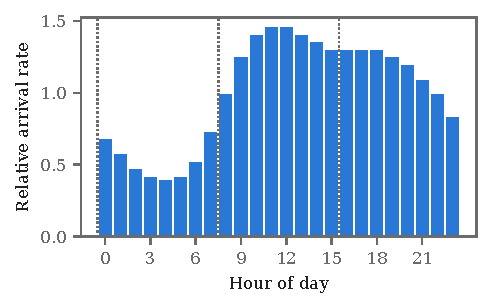
\includegraphics[width=0.8\columnwidth]{figures/fig_arrival_profile.pdf}
\caption{Hourly arrival profile (relative to the daily mean). Dotted lines: start of the night, day and evening physician shifts.}
\label{fig:profile}
\end{figure}

\subsection{Pathways}

Table~\ref{tab:pathways} lists the \NPathways{} published pathways \cite{Rismanchian2023_PatientJourney} with their published shares and the probability that a patient of a given CTAS level and disposition follows each of them in the model (typical diagnostic intensity). The probability of pathway $j$ for a patient of CTAS level $l$ with disposition $a$ is proportional to $f_j\exp\{(\theta_l+s)k_j\}$ over the pathways that end in $a$, where $f_j$ is the published frequency, $k_j$ the number of diagnostic and consultation steps, $\theta_l$ the CTAS tilt (from \TiltOneAll{} for CTAS~1 to \TiltFiveAll{} for CTAS~5) and $s$ the diagnostic-intensity shift.

\begin{table}[!htbp]
\centering
\caption{Published pathways and model probabilities by CTAS level, given the disposition in which the pathway ends (typical diagnostic intensity). TR triage, RG registration, AS physician assessment, LB laboratory, XR X-ray, DR consultation, DD discharge, AD admission.}
\label{tab:pathways}
\footnotesize
\begin{adjustbox}{max width=\linewidth}\begin{tabular}{llrrrr}
\toprule
 & & Published & \multicolumn{3}{c}{Model probability given disposition (\%)} \\
\cmidrule(lr){4-6}
Pathway & Steps & share (\%) & CTAS 1 & CTAS 3 & CTAS 5 \\
\midrule
V1 & TR-RG-AS-DD & 31.0 & 21.0 & 37.6 & 54.8 \\
V2 & TR-RG-AS-XR-DD & 16.0 & 17.9 & 19.4 & 17.1 \\
V3 & TR-RG-AS-LB-XR-DD & 10.9 & 20.1 & 13.2 & 7.1 \\
V4 & TR-RG-AS-CT-XR-DR-AD & 10.2 & 74.0 & 57.6 & 37.8 \\
V5 & TR-RG-AS-DR-DD & 10.1 & 11.3 & 12.2 & 10.8 \\
V6 & TR-RG-AS-LB-XR-DR-DD & 6.0 & 18.3 & 7.3 & 2.4 \\
V7 & TR-RG-AS-LB-AD & 4.1 & 11.0 & 23.2 & 41.4 \\
V8 & TR-RG-AS-XR-LB-AD & 3.4 & 15.0 & 19.2 & 20.8 \\
V9 & TR-RG-AS-LB-DD & 3.3 & 3.7 & 4.0 & 3.5 \\
V10 & TR-RG-AS-XR-LB-DD & 2.7 & 5.0 & 3.3 & 1.8 \\
V11 & TR-RG-AS-CT-DD & 2.4 & 2.7 & 2.9 & 2.6 \\
\bottomrule
\end{tabular}\end{adjustbox}
\end{table}

\subsection{Capacity Sizing and Load}

Let $\lambda_s$ be the arrival rate in shift $s$ at the base volume, and $\omega^{\text{hi}}$ and $\omega^{\text{lo}}$ the expected physician work per arriving patient contributed by CTAS~1--3 and CTAS~4--5 patients. The number of physicians in shift $s$ is
\begin{equation}
c_s=\big\lceil\lambda_s\omega^{\text{hi}}/\rho\big\rceil+\big\lceil\lambda_s\omega^{\text{lo}}/\rho\big\rceil,\qquad \rho=\PhysTargetMedium,
\end{equation}
and the second term is the fast-track team in the fast-track configuration. Treatment spaces are sized in the same way from the expected service-only holding time with $\rho=\SpaceSizing$, at the arrival rate that gives the medium load, and the CTAS~4--5 share forms the second area in the two-area configurations. Diagnostic resources are sized for an offered load of \DiagTarget{} and triage nurses for \TriageTarget{} at the busiest hour of the high load level. Finally the arrival rate is scaled so that the offered load of the busiest physician pool equals the load level (for the fast-track configuration, the larger of the Main and fast-track offered loads under CTAS streaming). Sensitivity and robustness experiments change demand-side inputs but keep these capacities.

\begin{table*}[!htbp]
\centering
\caption{Visits per day by load level, treatment spaces and physicians per shift (night/day/evening) for each acuity mix and configuration. Values in parentheses are the second area's share.}
\label{tab:capacity}
\footnotesize
\setlength{\tabcolsep}{5pt}
\begin{adjustbox}{max width=\linewidth}\begin{tabular}{llrrrrr}
\toprule
 & & \multicolumn{3}{c}{Visits per day} & Spaces & Physicians \\
\cmidrule(lr){3-5}
Acuity mix & Configuration & Low & Medium & High & (second area) & per shift (second area) \\
\midrule
Tertiary & Pooled & 229 & 262 & 295 & 41 & 4/10/9 \\
 & Fast track & 209 & 239 & 269 & 41 (5) & 4/10/9 (1/2/2) \\
 & Split flow & 229 & 262 & 295 & 41 (5) & 4/10/9 \\
\addlinespace
Community & Pooled & 218 & 249 & 280 & 35 & 4/9/7 \\
 & Fast track & 211 & 242 & 272 & 35 (9) & 4/9/7 (1/3/2) \\
 & Split flow & 218 & 249 & 280 & 35 (9) & 4/9/7 \\
\addlinespace
Urgent-care-like & Pooled & 233 & 267 & 300 & 31 & 4/8/7 \\
 & Fast track & 229 & 261 & 294 & 31 (15) & 4/8/7 (2/4/4) \\
 & Split flow & 233 & 267 & 300 & 31 (15) & 4/8/7 \\
\bottomrule
\end{tabular}\end{adjustbox}
\end{table*}

\subsection{Designs of the Robustness Experiments}

In E8 one input of a medium-load core ED type is changed at a time while all capacities stay as sized for the core inputs: physician activity times are multiplied by 0.9 or 1.1, diagnostic activity times by 0.75 or 1.25, every coefficient of variation by 0.5 or 1.5; the hourly arrival profile is replaced by a flat profile or by the core profile raised to the power 1.5 and renormalized (more peaked); or the predicted codes of a patient are drawn from one common uniform random number for all attributes, so that prediction errors are fully correlated across attributes.

In E9 the \NOosTypes{} ED types are drawn by Latin hypercube sampling in four dimensions, ten per configuration: an acuity position $t\in[0,1]$, which interpolates the CTAS shares linearly between the urgent-care-like ($t=0$), community ($t=0.5$) and tertiary ($t=1$) mixes; the offered load of the busiest physician pool in $[0.70,0.90]$; the mean boarding time in $[120,360]$ minutes; and a shift of the diagnostic tilt in $[-0.3,0.3]$. Capacities are sized for each ED type by the sizing rule above, and patient lists use their own random-number streams. The decision guide is applied with the acuity mix nearest to $t$ (urgent-care-like for $t<0.25$, tertiary for $t\geq0.75$), and the optimized rules are those of the nearest core ED type in acuity and load.

\subsection{Time Stamps and Measures}

The event log records, for every patient and activity, the time of request, start and end. The time stamps used by the measures are: arrival (door); start of triage; first start of a treatment space (bed or chair); start of the physician initial assessment; disposition decision (end of the last physician encounter); and departure (end of discharge process or boarding). Every patient who arrives in the observation window is followed to departure.

\subsection{Verification Tests}

The test suite (\texttt{sim/tests}) contains tests of: each queue rule on small deterministic queues; equality between the per-level heap implementation and a full scan of the queue for the dynamic rules (APQ, ageing); Propositions~1--4 by exhaustive enumeration of codes; every KPI function against a hand-computed example; patient conservation, the order of time stamps and the absence of capacity violations in full runs; determinism (same policy and seed give identical results); equality of the fast KPI path used in optimization with the event-log KPIs; equality of ED types built from names and from numeric inputs; and the reassessment bonus, routing offset and demand perturbations.

Before any table or figure is built, automated checks confirm that every observed patient departed, that rates and utilizations lie in $[0,1]$, that every overall mean lies within the range of its group means, and that runs shared between experiments give identical numbers (for example, $\alpha=1$ in E4 and E2, the default policy in E7 and E2, and the optimized rules in E6, E6b and E7). One script then builds every table, figure and number quoted in the paper from the raw output files, together with a provenance record of the code version, configuration, seeds and run settings, and a second script checks that the text contains no result typed by hand.

In E3 the engine runs the similarity index and, at every dispatch from a queue with at least two waiting patients, records whether the reference rule would have chosen the same patient (Algorithm~\ref{alg:fidelity}). At every fifth such dispatch with at least three waiting patients it also computes Kendall's $\tau$ between the two orderings of the whole queue. The reference rule is then run separately on the same patient list, and the two event logs and KPIs are compared.

\FloatBarrier
\section{Algorithms}
\label{app:algorithms}

This appendix gives the main algorithms in pseudo-code. Algorithm~\ref{alg:engine} is the event loop of the simulation, Algorithm~\ref{alg:queue} the queue used for every resource, and Algorithm~\ref{alg:fidelity} the decision-level fidelity measurement. The cross-entropy optimization is given in Algorithm~\mref{alg:cem} in Section~\mref{sec:optimization}.

\begin{algorithm}[H]
\caption{Event loop of the ED simulation}
\label{alg:engine}
\begin{algorithmic}[1]
\REQUIRE patient list (arrival times, CTAS, pathway, durations, predicted codes), ED type, queue rule, routing rule
\STATE schedule all arrivals and all shift changes; $n_{\text{obs}}\leftarrow$ number of patients arriving in the observation window
\WHILE{$n_{\text{obs}}>0$}
\STATE pop the earliest event $(t,\text{type},i)$; set the clock to $t$
\IF{arrival} \STATE request a triage nurse
\ELSIF{end of triage} \STATE release the nurse; schedule end of registration
\ELSIF{end of registration} \STATE route $i$ to Main or the second area; request a treatment space
\ELSIF{end of physician encounter} \STATE release the physician; release the chair if the area is vertical
\STATE \textbf{if} initial assessment and pathway has steps \textbf{then} request the first step \textbf{else} decide
\ELSIF{end of a pathway step} \STATE release the resource; request the next step, or a physician reassessment (and a chair in the vertical area)
\ELSIF{end of discharge process or boarding} \STATE release the space; record departure; \textbf{if} $i$ observed \textbf{then} $n_{\text{obs}}\leftarrow n_{\text{obs}}-1$
\ELSIF{shift change} \STATE set physician capacities (non-preemptive); dispatch physicians
\ENDIF
\ENDWHILE
\STATE \textbf{procedure} decide($i$): record the decision; discharged: schedule discharge process; admitted: schedule boarding (a vertical patient first requests a Main bed)
\STATE \textbf{procedure} request($r$, $i$): insert $i$ in the queue of $r$ (Algorithm~\ref{alg:queue}); dispatch $r$
\STATE \textbf{procedure} dispatch($r$): \textbf{while} $r$ has a free server and a non-empty queue: pop the next patient and start the activity; a free Main space with an empty Main queue may take a waiting fast-track patient
\end{algorithmic}
\end{algorithm}

\begin{algorithm}[H]
\caption{Queue ordered by a queue rule}
\label{alg:queue}
\begin{algorithmic}[1]
\REQUIRE rule with static key $\kappa(i)$ (order within a CTAS level) and dynamic key $\phi(\kappa,l,t)$ (comparison across levels at time $t$)
\STATE \textbf{insert}($i$): push $(\kappa(i),i)$ on the heap $H_l$ of the patient's CTAS level $l$; every key ends in (time joined, patient id)
\STATE \textbf{pop}($t$): \textbf{if} $H_1\neq\emptyset$ \textbf{then return} the head of $H_1$ \COMMENT{CTAS~1 first}
\STATE \quad $l^*\leftarrow\arg\min_{l\in\{2,\dots,5\},H_l\neq\emptyset}\phi(\kappa(\text{head}(H_l)),l,t)$; \textbf{return} the head of $H_{l^*}$
\STATE \textit{Examples:} CTAS: $\kappa=(t_0,i)$, $\phi=(l,\kappa)$. APQ: $\kappa=(t_0,i)$, $\phi=(-(t-t_0)/T_l,\kappa)$. Similarity with ageing $\gamma$ and bonus $\beta$: $\kappa=(-[S(p)+\beta\,\mathbb{1}_{\text{RA}}-\gamma t_0/T_l],t_0,i)$, $\phi=(\kappa_1-\gamma t/T_l,\dots)$
\end{algorithmic}
\end{algorithm}

Within one CTAS level the static key gives the same order as the effective priority at any time, because the ageing rate $\gamma/T_l$ is common to the level; only the heads of the five levels need to be compared at a dispatch. The test suite checks that this gives the same choice as a full scan of the queue.

\begin{algorithm}[H]
\caption{Decision-level fidelity of a similarity index $\sigma$ to a reference rule $\rho$}
\label{alg:fidelity}
\begin{algorithmic}[1]
\STATE run the simulation with $\sigma$; at every dispatch from a queue $Q$ with $|Q|\ge2$:
\STATE \quad $a\leftarrow$ patient chosen by $\sigma$; $b\leftarrow$ patient that $\rho$ would choose from the same $Q$ at the same time
\STATE \quad $n\leftarrow n+1$; \textbf{if} $a=b$ \textbf{then} $m\leftarrow m+1$
\STATE \quad at every fifth such dispatch with $|Q|\ge3$: record Kendall's $\tau$ between the orders of $Q$ under $\sigma$ and $\rho$
\STATE agreement $=m/n$; also run $\rho$ alone on the same patients and compare the event logs and KPIs
\end{algorithmic}
\end{algorithm}

\FloatBarrier
\section{Additional Results}
\label{app:results}

This appendix reports the detailed results behind the summaries in Section~\mref{sec:results}. All values are generated from the simulation output by the scripts in the repository; the files in the \texttt{paper/supplement} folder contain the same results in machine-readable form.

\subsection{Face Validity}
\label{app:res:face}

Table~\ref{tab:face} gives the time intervals of the community, pooled ED under the default policy at the three load levels, which Section~\mref{sec:res:vv} compares with published Canadian values.

\begin{table}[!ht]
\centering
\caption{Face validity: community ED, pooled configuration, default policy, \Reps{} replications per load level.}
\label{tab:face}
\footnotesize
\begin{adjustbox}{max width=\linewidth}\begin{tabular}{lrrr}
\toprule
Measure (h unless stated) & Low & Medium & High \\
\midrule
Door to physician, median & 0.2 & 0.2 & 0.4 \\
Door to physician, P90 & 0.4 & 0.8 & 3.4 \\
LOS discharged, median & 1.5 & 1.6 & 2.1 \\
LOS discharged, P90 & 3.2 & 3.7 & 6.2 \\
LOS CTAS 4, P90 & 3.5 & 4.7 & 8.9 \\
LOS admitted, median & 4.9 & 5.1 & 5.4 \\
LOS admitted, P90 & 9.1 & 9.4 & 10.3 \\
Physician utilisation & 0.70 & 0.80 & 0.90 \\
Space utilisation & 0.54 & 0.67 & 0.85 \\
\bottomrule
\end{tabular}\end{adjustbox}
\end{table}

\subsection{Best Policy by ED Type}
\label{app:res:best}

Table~\ref{tab:best} lists, for every core ED type, the default policy and the best policy for RATP and mean LOS, with the number of policies that are statistically tied with the best. Table~\ref{tab:kpis} and Fig.~\ref{fig:tails} give the full set of measures for one ED type, the community ED at high load.

\begin{table*}[!t]
\centering
\caption{Default policy and best policy by ED type (\Reps{} replications). Tied: number of policies whose paired difference from the best is not significant at the 95\% level, out of all policies for the configuration.}
\label{tab:best}
\scriptsize
\setlength{\tabcolsep}{3pt}
\begin{adjustbox}{max width=\linewidth}\begin{tabular}{lllrlrr lrr}
\toprule
 & & & \multicolumn{4}{c}{RATP} & \multicolumn{3}{c}{Mean LOS (min)} \\
\cmidrule(lr){4-7}\cmidrule(lr){8-10}
Acuity & Load & Config. & Default & Best policy & Best & Tied & Best policy & Best & Default \\
\midrule
Tertiary & low & Pooled & 0.38 & SIM & 0.36 & 1/7 & FCFS & 154 & 155 \\
 &  & Fast track & 0.44 & SIM/S & 0.38 & 5/21 & FCFS/S & 154 & 155 \\
 &  & Split flow & 0.37 & SIM/S & 0.35 & 2/21 & FCFS/C & 154 & 155 \\
\addlinespace[1pt]
 & medium & Pooled & 0.60 & SIM & 0.53 & 1/7 & SIM & 166 & 168 \\
 &  & Fast track & 0.64 & SIM/S & 0.50 & 1/21 & FCFS/S & 162 & 168 \\
 &  & Split flow & 0.58 & SIM/S & 0.50 & 1/21 & FCFS/S & 165 & 167 \\
\addlinespace[1pt]
 & high & Pooled & 1.09 & SIM & 0.89 & 1/7 & SIM & 204 & 229 \\
 &  & Fast track & 1.02 & SIM/S & 0.76 & 1/21 & SIM/S & 179 & 203 \\
 &  & Split flow & 0.96 & SIM/S & 0.80 & 2/21 & SIM-AGE/S & 193 & 206 \\
\addlinespace[1pt]
Community & low & Pooled & 0.38 & CTAS-PD & 0.37 & 5/7 & FCFS & 138 & 138 \\
 &  & Fast track & 0.55 & SIM/S & 0.47 & 1/21 & SIM/C & 143 & 144 \\
 &  & Split flow & 0.37 & CTAS-SPT/S & 0.36 & 3/21 & FCFS/S & 138 & 138 \\
\addlinespace[1pt]
 & medium & Pooled & 0.60 & SIM & 0.56 & 1/7 & SIM & 151 & 155 \\
 &  & Fast track & 0.83 & SIM/S & 0.65 & 1/21 & SIM/C & 157 & 159 \\
 &  & Split flow & 0.59 & CTAS-SPT/S & 0.53 & 3/21 & SIM/S & 150 & 154 \\
\addlinespace[1pt]
 & high & Pooled & 1.05 & SIM & 0.92 & 1/7 & SIM & 195 & 213 \\
 &  & Fast track & 1.31 & SIM/S & 1.07 & 1/21 & SIM/S & 199 & 212 \\
 &  & Split flow & 0.96 & CTAS-SPT/S & 0.84 & 3/21 & FCFS/S & 187 & 202 \\
\addlinespace[1pt]
Urgent-care-like & low & Pooled & 0.30 & CTAS & 0.30 & 3/7 & SIM & 119 & 120 \\
 &  & Fast track & 0.77 & SIM/S & 0.53 & 5/21 & FCFS/S & 126 & 128 \\
 &  & Split flow & 0.41 & CTAS/S & 0.37 & 5/21 & SIM/S & 120 & 120 \\
\addlinespace[1pt]
 & medium & Pooled & 0.57 & CTAS-SPT & 0.55 & 4/7 & SIM & 130 & 135 \\
 &  & Fast track & 1.15 & SIM/S & 0.83 & 2/21 & SIM/S & 140 & 149 \\
 &  & Split flow & 0.68 & CTAS/S & 0.63 & 4/21 & FCFS/S & 131 & 134 \\
\addlinespace[1pt]
 & high & Pooled & 0.92 & CTAS-SPT & 0.87 & 3/7 & SIM & 165 & 192 \\
 &  & Fast track & 1.55 & CTAS-SPT/S & 1.28 & 4/21 & SIM/S & 189 & 223 \\
 &  & Split flow & 1.00 & CTAS-SPT/C & 0.93 & 5/21 & FCFS/S & 163 & 172 \\
\bottomrule
\end{tabular}\end{adjustbox}
\end{table*}

\begin{table*}[!ht]
\centering
\caption{Performance by queue rule in the community ED at high load (pooled; \Reps{} replications). Second line of each measure: paired difference from CTAS; bold if the 95\% confidence interval excludes zero.}
\label{tab:kpis}
\footnotesize
\begin{adjustbox}{max width=\linewidth}\begin{tabular}{lrrrrrrr}
\toprule
KPI & FCFS & CTAS & APQ & CTAS-SPT & CTAS-PD & SIM & SIM-AGE \\
\midrule
RATP & 1.145 & 1.046 & 1.177 & 0.982 & 1.009 & 0.918 & 1.031 \\
\quad vs CTAS & \textbf{+0.099} & -- & \textbf{+0.130} & \textbf{-0.064} & \textbf{-0.037} & \textbf{-0.128} & -0.015 \\
AWT (min) & 48.3 & 89.2 & 54.6 & 85.6 & 89.9 & 50.1 & 49.8 \\
\quad vs CTAS & \textbf{-41.0} & -- & \textbf{-34.6} & \textbf{-3.6} & +0.6 & \textbf{-39.1} & \textbf{-39.4} \\
P90 door to physician (min) & 147 & 206 & 164 & 152 & 185 & 102 & 150 \\
\quad vs CTAS & \textbf{-59} & -- & \textbf{-42} & \textbf{-53} & \textbf{-20} & \textbf{-104} & \textbf{-56} \\
P95 door to physician, CTAS 2 (min) & 194 & 31 & 86 & 31 & 31 & 101 & 77 \\
\quad vs CTAS & \textbf{+163} & -- & \textbf{+55} & -0 & +0 & \textbf{+70} & \textbf{+46} \\
P95 door to physician, CTAS 5 (min) & 188 & 1289 & 594 & 1328 & 1320 & 654 & 700 \\
\quad vs CTAS & \textbf{-1101} & -- & \textbf{-695} & +39 & +31 & \textbf{-635} & \textbf{-589} \\
Mean LOS (min) & 197.7 & 212.9 & 203.3 & 207.5 & 211.9 & 195.0 & 196.0 \\
\quad vs CTAS & \textbf{-15.2} & -- & \textbf{-9.6} & \textbf{-5.5} & \textbf{-1.0} & \textbf{-18.0} & \textbf{-16.9} \\
Mean LOS, discharged (min) & 160.9 & 184.1 & 170.2 & 176.8 & 179.7 & 146.3 & 156.8 \\
\quad vs CTAS & \textbf{-23.3} & -- & \textbf{-14.0} & \textbf{-7.3} & \textbf{-4.4} & \textbf{-37.8} & \textbf{-27.3} \\
Mean LOS, admitted (min) & 412.6 & 381.2 & 396.9 & 386.4 & 399.8 & 478.7 & 424.8 \\
\quad vs CTAS & \textbf{+31.4} & -- & \textbf{+15.7} & \textbf{+5.3} & \textbf{+18.7} & \textbf{+97.5} & \textbf{+43.6} \\
\bottomrule
\end{tabular}\end{adjustbox}
\end{table*}

\begin{figure}[!ht]
\centering
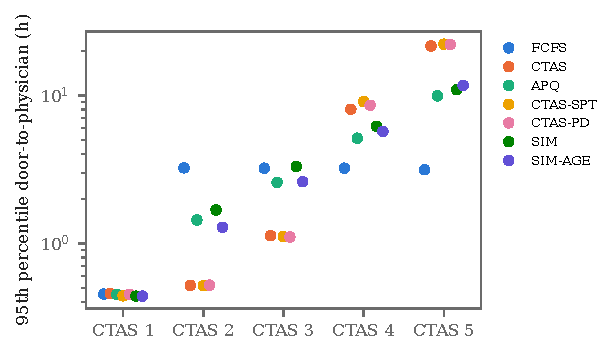
\includegraphics[width=0.95\columnwidth]{figures/fig_tails.pdf}
\caption{95th percentile of door-to-physician time by CTAS level and queue rule (community ED, high load, pooled; log scale).}
\label{fig:tails}
\end{figure}

\subsection{How Firmly Is the Best Policy Identified?}
\label{app:res:boot}

For each ED type and measure we drew \BootB{} bootstrap samples of the \Reps{} replications (resampling replications, so that the pairing of policies on common random numbers is kept) and recorded which policy had the lowest mean in each sample. For RATP the policy that is best on the full sample remains best in a median of \BootRatpMedianP\% of the bootstrap samples; the share is at least 90\% in \BootRatpNNinety{} of the \NEdTypes{} ED types and below one half in \BootRatpNHalf. For mean LOS the median is \BootLosMedianP\% (at least 90\% in \BootLosNNinety{} ED types, below one half in \BootLosNHalf). Where the share is low, two or more policies are practically equivalent, which is consistent with the ties reported in Table~\ref{tab:best}; the regret of choosing any of them is then small.

\subsection{Alternative Acuity Weights in RATP}
\label{app:res:altw}

RATP weights the breach rate of CTAS level $l$ by $1/l$. Table~\ref{tab:altw} repeats the identification of the best policy per ED type and of the best single policy with three other weightings. With linear weights $6-l$, the best policy is unchanged in \AltWLinearSame{} of the \NEdTypes{} ED types; with equal weights in \AltWEqualSame{}; and with inverse-square weights in \AltWSteepSame. Equal weights give the breach rate of all patients and therefore put most weight on CTAS~3 and~4, which are the largest groups.

\begin{table}[!t]
\centering
\caption{Best policies under alternative acuity weights for the breach-rate measure. Same best: number of ED types in which the best policy equals the best policy under RATP. Best single policy: the policy with the smallest mean regret over all ED types.}
\label{tab:altw}
\footnotesize
\begin{adjustbox}{max width=\linewidth}\begin{tabular}{lrlrr}
\toprule
Acuity weights & Same best as RATP & Best single policy & Mean regret (\%) & Max regret (\%) \\
\midrule
$1/l$ (RATP) & 27/27 & CTAS-SPT/S & 2.8 & 13.5 \\
$6-l$ & 25/27 & CTAS-SPT/S & 2.3 & 13.6 \\
equal & 18/27 & SIM/S & 1.7 & 14.5 \\
$1/l^2$ & 17/27 & CTAS-SPT/S & 1.8 & 5.3 \\
\bottomrule
\end{tabular}\end{adjustbox}
\end{table}

\subsection{Sensitivity to Boarding and Diagnostic Intensity}
\label{app:res:sens}

Table~\ref{tab:sens} reports the sensitivity analysis summarized in Section~\mref{sec:res:sens}. The supplement contains the results for every policy and ED type, and those of the value-of-prediction experiment.

\begin{table}[!ht]
\centering
\caption{Sensitivity (\NMediumTypes{} medium-load ED types, \RepsSecondary{} replications): number of ED types in which the core best policy is still best, and mean (maximum) regret of keeping the core best policy.}
\label{tab:sens}
\footnotesize
\setlength{\tabcolsep}{3pt}
\begin{adjustbox}{max width=\linewidth}\begin{tabular}{lrrrr}
\toprule
 & \multicolumn{2}{c}{RATP} & \multicolumn{2}{c}{Mean LOS} \\
\cmidrule(lr){2-3}\cmidrule(lr){4-5}
Variant & Same best & Regret of core best (\%) & Same best & Regret of core best (\%) \\
\midrule
High boarding & 5/9 & 1.0 (max 4.6) & 5/9 & 2.3 (max 12.7) \\
Light diagnostics & 6/9 & 0.5 (max 2.1) & 4/9 & 0.1 (max 0.5) \\
Heavy diagnostics & 5/9 & 5.7 (max 32.3) & 4/9 & 11.7 (max 83.0) \\
\bottomrule
\end{tabular}\end{adjustbox}
\end{table}

\subsection{Trade-Offs and Value of Prediction}
\label{app:res:vop}

Fig.~\ref{fig:pareto} shows mean LOS against RATP for all policies in the community ED at high load, and Table~\ref{tab:vop} the gain of the best prediction-based policy over the best policy without predictions in the medium-load ED types (Sections~\mref{sec:res:mech} and~\mref{sec:res:vop}).

\begin{figure}[!ht]
\centering
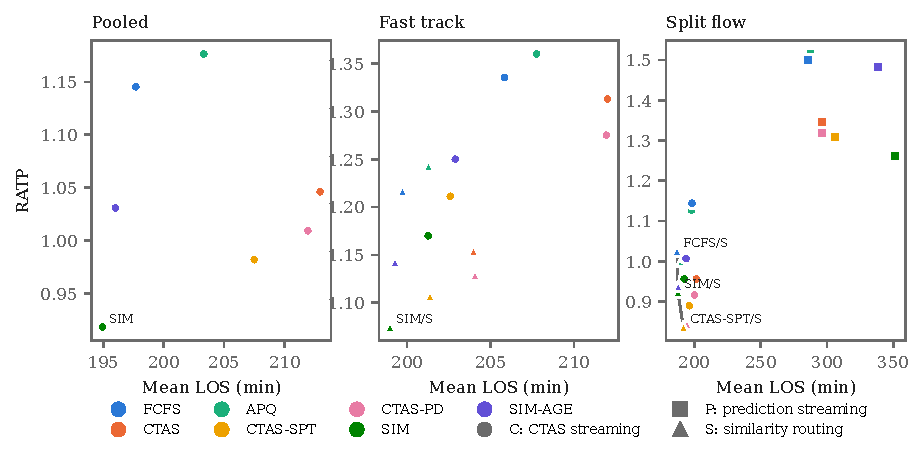
\includegraphics[width=\columnwidth]{figures/fig_pareto.pdf}
\caption{Mean LOS against RATP for all policies in the community ED at high load. Grey line: policies not dominated on both measures (labelled). Overloaded policies (Main-area utilization $\geq$ \OverloadThreshold) are omitted.}
\label{fig:pareto}
\end{figure}

\begin{table*}[!ht]
\centering
\caption{Gain of the best prediction-based policy over the best policy without predictions (medium load), with perfect information ($\alpha=0$) and reference accuracy ($\alpha=1$), and the largest $\alpha$ tested at which it is still better ($\geq$: better at every $\alpha$ tested).}
\label{tab:vop}
\footnotesize
\setlength{\tabcolsep}{2.5pt}
\begin{adjustbox}{max width=\linewidth}\begin{tabular}{llrrrrrr}
\toprule
 & & \multicolumn{3}{c}{RATP} & \multicolumn{3}{c}{Mean LOS} \\
\cmidrule(lr){3-5}\cmidrule(lr){6-8}
Acuity & Config. & Gain $\alpha{=}0$ (\%) & Gain $\alpha{=}1$ (\%) & Max $\alpha$ & Gain $\alpha{=}0$ (\%) & Gain $\alpha{=}1$ (\%) & Max $\alpha$ \\
\midrule
Tertiary & Pooled & 12.7 & 11.1 & $\geq$1.50 & 1.2 & 1.0 & $\geq$1.50 \\
 & Fast track & 23.3 & 21.5 & $\geq$1.50 & 3.6 & 3.3 & $\geq$1.50 \\
 & Split flow & 12.9 & 11.9 & $\geq$1.50 & 1.1 & 1.1 & $\geq$1.50 \\
Community & Pooled & 11.3 & 7.4 & $\geq$1.50 & 1.8 & 1.6 & $\geq$1.50 \\
 & Fast track & 21.2 & 20.9 & $\geq$1.50 & 0.8 & 0.8 & $\geq$1.50 \\
 & Split flow & 11.5 & 11.5 & $\geq$1.50 & 1.9 & 1.8 & $\geq$1.50 \\
Urgent-care-like & Pooled & 0.9 & 0.6 & 1.50 & 2.6 & 2.5 & $\geq$1.50 \\
 & Fast track & 22.4 & 25.9 & $\geq$1.50 & 2.6 & 5.0 & $\geq$1.50 \\
 & Split flow & 4.1 & 7.0 & 1.50 & 1.7 & 2.0 & $\geq$1.50 \\
\bottomrule
\end{tabular}\end{adjustbox}
\end{table*}

\subsection{Optimized Similarity Rules: Details}
\label{app:res:opt}

Table~\ref{tab:optfull} gives the test-replication objective of the default policy, the best fixed policy and the optimized similarity policy for every ED type. The best fixed policy is the one with the lowest mean objective on the same test replications, so the comparison is conservative for the optimized rule: the fixed policy is selected with knowledge of the test outcomes, the optimized rule is not. Fig.~\ref{fig:optparamsaccess} shows the parameters of the rules optimized for the access objective (Fig.~\mref{fig:optparams} in the main text shows the balanced objective) and Fig.~\ref{fig:cem} the progress of the search. On average, the training objective of the selected rule was \OptAccessTrainOptimism\% (access) and \OptBalancedTrainOptimism\% (balanced) away from its test value and the validation objective \OptAccessValOptimism\% and \OptBalancedValOptimism\%; negative values mean the search replications were more favourable than the test replications. Each search used about \CemEvalsPerType{} simulation runs per ED type and objective. Table~\ref{tab:levers} gives the lever check of experiment E6b and Fig.~\ref{fig:transfer} the transfer regret of every pair of ED types.

\begin{table*}[!t]
\centering
\caption{Objective on the \Reps{} test replications by ED type: default policy (CTAS/C), best fixed policy, and optimized similarity policy. Balanced objective: $J=\tfrac12\,\text{RATP}/\text{RATP}_0+\tfrac12\,\overline{\text{LOS}}/\overline{\text{LOS}}_0$, so $J=1$ for the default policy. $^{*}$: optimized better than the best fixed policy (paired 95\% confidence interval excludes zero); $^{\dagger}$: worse.}
\label{tab:optfull}
\scriptsize
\setlength{\tabcolsep}{3pt}
\begin{adjustbox}{max width=\linewidth}\begin{tabular}{lllrrrlrrr}
\toprule
 & & & \multicolumn{3}{c}{Access (RATP)} & \multicolumn{4}{c}{Balanced ($J$)} \\
\cmidrule(lr){4-6}\cmidrule(lr){7-10}
Acuity & Load & Config. & Default & Best fixed & Optimized & Best fixed policy & Default & Best fixed & Optimized \\
\midrule
Tertiary & low & Pooled & 0.375 & 0.359 & 0.350$^{*}$ & SIM & 1.000 & 0.977 & 0.971 \\
 &  & Fast track & 0.441 & 0.382 & 0.364$^{*}$ & SIM/S & 1.000 & 0.930 & 0.916$^{*}$ \\
 &  & Split flow & 0.372 & 0.350 & 0.331$^{*}$ & SIM/S & 1.000 & 0.970 & 0.953$^{*}$ \\
 & medium & Pooled & 0.598 & 0.532 & 0.520$^{*}$ & SIM & 1.000 & 0.938 & 0.934 \\
 &  & Fast track & 0.637 & 0.498 & 0.490 & SIM/S & 1.000 & 0.873 & 0.870 \\
 &  & Split flow & 0.576 & 0.504 & 0.436$^{*}$ & SIM/S & 1.000 & 0.931 & 0.902$^{*}$ \\
 & high & Pooled & 1.093 & 0.889 & 0.836$^{*}$ & SIM & 1.000 & 0.854 & 0.832$^{*}$ \\
 &  & Fast track & 1.023 & 0.758 & 0.733$^{*}$ & SIM/S & 1.000 & 0.813 & 0.799$^{*}$ \\
 &  & Split flow & 0.964 & 0.801 & 0.569$^{*}$ & SIM/S & 1.000 & 0.885 & 0.837$^{*}$ \\
Community & low & Pooled & 0.375 & 0.371 & 0.358$^{*}$ & CTAS-SPT & 1.000 & 0.996 & 0.984 \\
 &  & Fast track & 0.555 & 0.467 & 0.457 & SIM/S & 1.000 & 0.938 & 0.923$^{*}$ \\
 &  & Split flow & 0.372 & 0.356 & 0.326$^{*}$ & CTAS-SPT/S & 1.000 & 0.980 & 0.954$^{*}$ \\
 & medium & Pooled & 0.603 & 0.561 & 0.554 & SIM & 1.000 & 0.953 & 0.952 \\
 &  & Fast track & 0.828 & 0.654 & 0.628$^{*}$ & SIM/S & 1.000 & 0.893 & 0.887 \\
 &  & Split flow & 0.594 & 0.527 & 0.418$^{*}$ & CTAS-SPT/S & 1.000 & 0.939 & 0.872$^{*}$ \\
 & high & Pooled & 1.046 & 0.918 & 0.897 & SIM & 1.000 & 0.897 & 0.877$^{*}$ \\
 &  & Fast track & 1.313 & 1.075 & 0.999$^{*}$ & SIM/S & 1.000 & 0.879 & 0.833$^{*}$ \\
 &  & Split flow & 0.957 & 0.837 & 0.529$^{*}$ & CTAS-SPT/S & 1.000 & 0.914 & 0.777$^{*}$ \\
Urgent-care-like & low & Pooled & 0.301 & 0.301 & 0.319 & CTAS & 1.000 & 1.000 & 1.035 \\
 &  & Fast track & 0.766 & 0.532 & 0.493 & SIM/S & 1.000 & 0.839 & 0.836 \\
 &  & Split flow & 0.412 & 0.368 & 0.277$^{*}$ & CTAS/S & 1.000 & 0.960 & 0.843$^{*}$ \\
 & medium & Pooled & 0.566 & 0.547 & 0.573 & CTAS-SPT & 1.000 & 0.985 & 1.000 \\
 &  & Fast track & 1.151 & 0.828 & 0.772$^{*}$ & SIM/S & 1.000 & 0.830 & 0.817 \\
 &  & Split flow & 0.680 & 0.631 & 0.412$^{*}$ & CTAS-PD/S & 1.000 & 0.962 & 0.808$^{*}$ \\
 & high & Pooled & 0.923 & 0.874 & 0.873 & SIM & 1.000 & 0.913 & 0.903 \\
 &  & Fast track & 1.547 & 1.276 & 1.145$^{*}$ & SIM/S & 1.000 & 0.846 & 0.759$^{*}$ \\
 &  & Split flow & 1.001 & 0.930 & 0.479$^{*}$ & CTAS-SPT/C & 1.000 & 0.952 & 0.736$^{*}$ \\
\bottomrule
\end{tabular}\end{adjustbox}
\end{table*}

\begin{figure*}[!t]
\centering
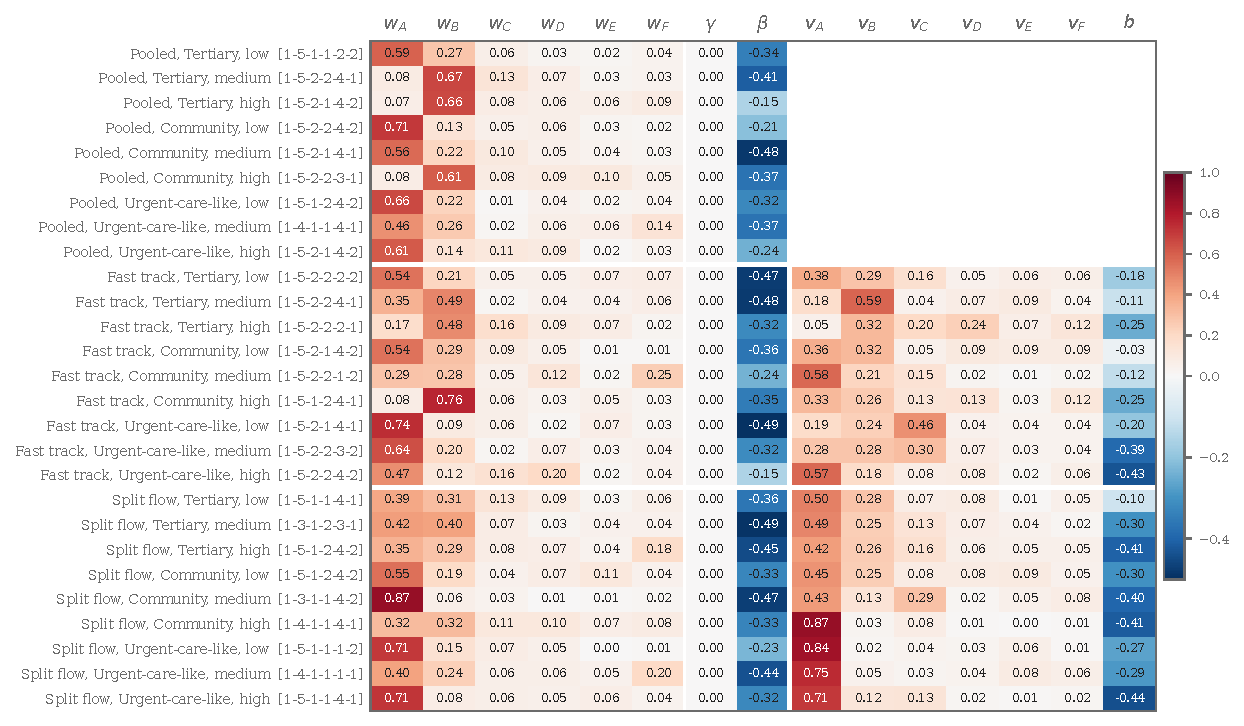
\includegraphics[width=\textwidth]{figures/fig_opt_params_access.pdf}
\caption{Parameters of the similarity rules optimized for the access objective. Rows: ED types, with the optimized target code $q_A$--$q_F$ in brackets. Columns: queue weights, ageing $\gamma$, reassessment bonus $\beta$, routing weights and routing offset $b$ (two-area EDs only).}
\label{fig:optparamsaccess}
\end{figure*}

\begin{figure}[!t]
\centering
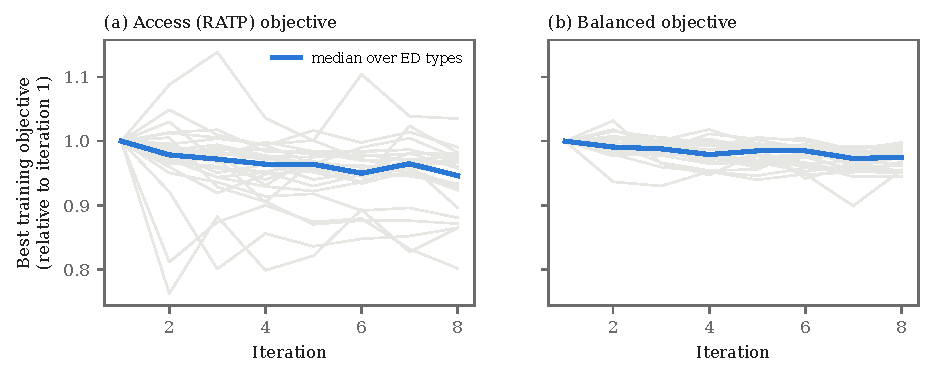
\includegraphics[width=\columnwidth]{figures/fig_cem_convergence.pdf}
\caption{Best training objective by iteration of the cross-entropy search, relative to the first iteration. Grey: individual ED types; blue: median.}
\label{fig:cem}
\end{figure}

\begin{table}[!ht]
\centering
\caption{Change in the objective (\%) when one parameter of the optimized rule is changed (E6b, \NLeverReps{} test replications); negative is better. Better/worse: ED types with a change of more than 1\% in either direction.}
\label{tab:levers}
\footnotesize
\begin{adjustbox}{max width=\linewidth}\begin{tabular}{lrrrrrr}
\toprule
 & \multicolumn{3}{c}{Access objective} & \multicolumn{3}{c}{Balanced objective} \\
\cmidrule(lr){2-4}\cmidrule(lr){5-7}
Change to the optimized rule & Mean change (\%) & Better & Worse & Mean change (\%) & Better & Worse \\
\midrule
Ageing $\gamma=0.02$ & +2.0 & 4/27 & 11/27 & +0.6 & 4/27 & 6/27 \\
Ageing $\gamma=0.05$ & +4.3 & 2/27 & 18/27 & +1.4 & 3/27 & 13/27 \\
Ageing $\gamma=0.1$ & +7.9 & 2/27 & 22/27 & +3.2 & 3/27 & 18/27 \\
Ageing $\gamma=0.2$ & +11.3 & 2/27 & 23/27 & +4.5 & 1/27 & 19/27 \\
Ageing $\gamma=0.4$ & +14.6 & 0/27 & 24/27 & +6.5 & 2/27 & 22/27 \\
No reassessment bonus ($\beta=0$) & +6.1 & 1/27 & 22/27 & +0.4 & 4/27 & 12/27 \\
No routing offset ($b=0$) & +4.4 & 4/18 & 12/18 & +2.6 & 2/18 & 7/18 \\
\bottomrule
\end{tabular}\end{adjustbox}
\end{table}

\begin{figure*}[!ht]
\centering
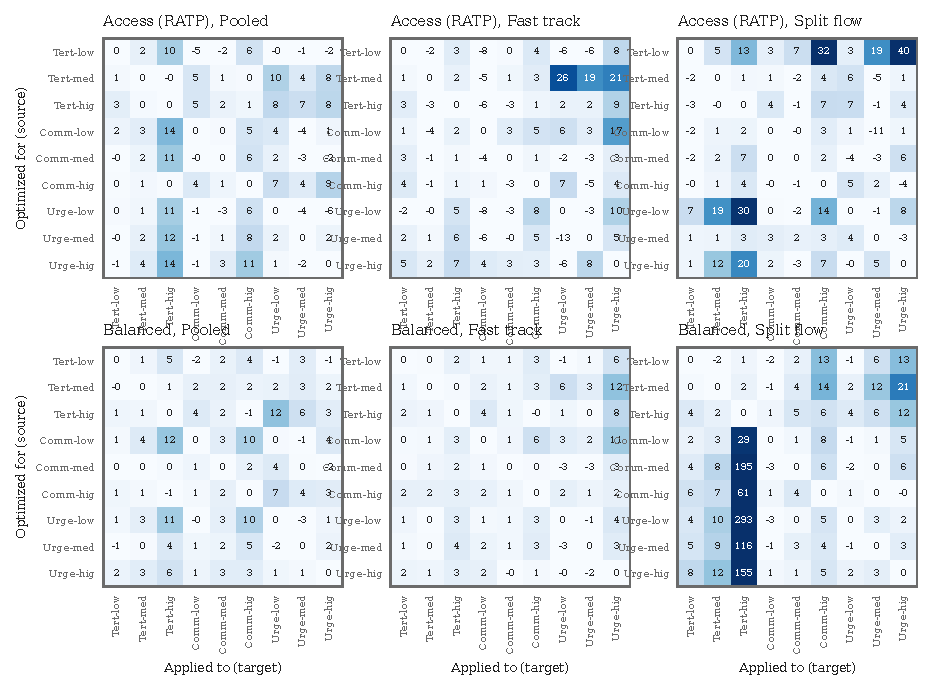
\includegraphics[width=0.95\textwidth]{figures/fig_transfer.pdf}
\caption{Transfer regret (\%) of optimized rules (\NTransferReps{} test replications). Row: ED type for which the rule was optimized; column: ED type to which it is applied; the diagonal is zero by definition. Top: access objective; bottom: balanced objective.}
\label{fig:transfer}
\end{figure*}

\subsection{Robustness to Misspecified Inputs: Details}
\label{app:res:rob}

Table~\ref{tab:rob} reports, for each perturbation in E8, the rank correlation between the policy ranking under the perturbed inputs and the ranking in the core design, the regret of the policy that was best in the core design when it is used under the perturbed inputs, and the balanced objective of the optimized rule relative to the best fixed policy under the perturbed inputs and to the default. Values are averages over the nine medium-load ED types.

\begin{table*}[!t]
\centering
\caption{Robustness of the policy ranking to misspecified inputs (medium-load ED types, \NRobReps{} replications). Kendall $\tau$: rank correlation of mean RATP or mean LOS over all fixed policies between the perturbed and the core inputs. Regret of core best: regret under the perturbed inputs of the policy that is best under the core inputs. Optimized (balanced): balanced objective of the rule optimized under the core inputs, relative to the best fixed policy under the perturbed inputs (positive: worse) and improvement over the default.}
\label{tab:rob}
\footnotesize
\begin{adjustbox}{max width=\linewidth}\begin{tabular}{lrrrrrr}
\toprule
 & \multicolumn{2}{c}{Kendall $\tau$ of policy ranking} & \multicolumn{2}{c}{Regret of core best (\%)} & \multicolumn{2}{c}{Optimized (balanced)} \\
\cmidrule(lr){2-3}\cmidrule(lr){4-5}\cmidrule(lr){6-7}
Perturbation & RATP & LOS & RATP & LOS & vs best fixed (\%) & vs default (\%) \\
\midrule
Physician times $-10\%$ & 0.85 & 0.89 & 1.3 & 0.0 & -3.0 & 9.6 \\
Physician times $+10\%$ & 0.84 & 0.81 & 0.5 & 0.6 & -2.8 & 12.5 \\
Diagnostic times $-25\%$ & 0.83 & 0.70 & 0.9 & 0.1 & -0.9 & 8.2 \\
Diagnostic times $+25\%$ & 0.84 & 0.80 & 3.0 & 0.7 & -7.7 & 17.9 \\
All CVs $\times0.5$ & 0.86 & 0.90 & 1.1 & 0.0 & -3.3 & 12.5 \\
All CVs $\times1.5$ & 0.85 & 0.88 & 1.5 & 0.1 & -3.1 & 10.8 \\
Flat arrival profile & 0.75 & 0.64 & 1.9 & 0.8 & -0.5 & 7.0 \\
Peaked arrival profile & 0.87 & 0.87 & 1.7 & 0.2 & -5.1 & 14.2 \\
Correlated prediction errors & 0.84 & 0.89 & 2.5 & 0.3 & -2.7 & 9.8 \\
\bottomrule
\end{tabular}\end{adjustbox}
\end{table*}

\FloatBarrier


\bibliographystyle{\ifdefined\localbst unsrtnat\else IEEEtranN\fi}
\bibliography{ed_library}
\end{document}
